% Appendix D

\chapter{Additional Tables and Figures} % Main appendix title

\label{AppendixD} % For referencing this appendix elsewhere, use \ref{AppendixA}

\section{Tables}

\begin{table}[H]
\caption{Polynomial regression result for the European call option}
\label{tab:fullEuroCall}
\centering
\begin{tabular}{llllllll}
\toprule
\textbf{Data set} &  \textbf{Measure} & \textbf{1. degree} & \textbf{2. degree} & \textbf{3. degree} & {4. degree} & \textbf{5. degree} & {6. degree}\\
\midrule
In-Sample     &	MSE  & 0.000636 & 0.000069 & 0.000013 & 0.000004 & 0.000002 & 0.000001 \\
		      & RMSE & 0.025212 & 0.008316 & 0.003624 & 0.002052 & 0.001414 & 0.000958 \\
		      & MAE  & 0.018326 & 0.006141 & 0.002561 & 0.001280 & 0.000867 & 0.000591 \\
		      & $R^2$& 0.936628 & 0.993105 & 0.998691 & 0.999580 & 0.999801 & 0.999909 \\
Long Maturity & MSE  & 0.002662 & 0.001196 & 0.001654 & 0.003956 & 0.012255 & 0.043361 \\
		      & RMSE & 0.051593 & 0.034577 & 0.040666 & 0.062894 & 0.110702 & 0.208233 \\
		      & MAE  & 0.041232 & 0.026287 & 0.028371 & 0.039932 & 0.064402 & 0.111190 \\
		      & $R^2$& 0.818143 & 0.918316 & 0.887014 & 0.729744 & 0.162742 & -1.962442 \\
Out-of-Money  & MSE  & 0.005772 & 0.000767 & 0.000839 & 0.000944 & 0.001812 & 0.004423 \\
		      & RMSE & 0.075973 & 0.027694 & 0.028960 & 0.030724 & 0.042568 & 0.066506 \\
		      & MAE  & 0.060936 & 0.022203 & 0.020288 & 0.020542 & 0.027125 & 0.041315\\
		      & $R^2$& -2.377251 & 0.551246 & 0.509280 & 0.447668 & -0.060261 & -1.588030\\
\bottomrule\\
\end{tabular}
\end{table}

\begin{table}[H]
\caption{Hyperparameter tuning of dataset size and batchsize for american put minimum two assets for the interested reader see the tensorboard}
\label{tab:fullhyperAmerMin4}
\centering
\begin{tabular}{llll}
\toprule
\textbf{Data set Size} & \textbf{$\eta$} & \textbf{Batch Size} & \textbf{Loss} \\
\midrule
300K    & 0.0001 & 8     & 0.015130897983909 \\ 
300K    & 0.001  & 64    & 0.035523075610399 \\ 
100K    & 0.0001 & 8     & 0.064886227250099 \\ 
100K    & 0.001  & 8     & 0.072143875062466 \\ 
300K    & 0.0001 & 64    & 0.075988814234734 \\ 
300K    & 0.001  & 8     & 0.104622706770897 \\ 
300K    & 0.01   & 256   & 0.480043411254883 \\ 
300K    & 0.0001 & 256   & 1.04093873500824  \\ 
300K    & 0.001  & 256   & 1.06809389591217  \\ 
300K    & 0.001  & 512   & 1.08942472934723  \\ 
100K    & 0.001  & 64    & 1.18230485916138  \\ 
300K    & 0.001  & 1024  & 1.30065310001373  \\ 
300K    & 0.01   & 512   & 1.45135951042175  \\ 
100K    & 0.01   & 256   & 1.52623510360718  \\ 
300K    & 0.01   & 64    & 1.75954759120941  \\ 
300K    & 0.01   & 1024  & 1.92213356494904  \\ 
100K    & 0.01   & 512   & 2.01193928718567  \\ 
100K    & 0.01   & 64    & 2.02969717979431  \\ 
300K    & 0.0001 & 1024  & 5.72439670562744  \\ 
300K    & 0.0001 & 512   & 5.72847843170166  \\ 
100K    & 0.0001 & 256   & 5.76278400421143  \\ 
100K    & 0.0001 & 512   & 5.77397203445435  \\ 
100K    & 0.0001 & 64    & 5.80239868164063  \\ 
100K    & 0.0001 & 1024  & 5.90070772171021  \\ 
100K    & 0.001  & 256   & 6.29003953933716  \\ 
100K    & 0.001  & 512   & 6.52896738052368  \\ 
100K    & 0.001  & 1024  & 6.56187915802002  \\ 
1K      & 0.001  & 8     & 7.5845251083374   \\ 
100K    & 0.01   & 8     & 8.07239627838135  \\ 
1K      & 0.01   & 8     & 11.7414264678955  \\ 
100K    & 0.01   & 1024  & 13.4287099838257  \\ 
1K      & 0.01   & 64    & 14.1254253387451  \\ 
1K      & 0.0001 & 8     & 24.0087566375732  \\ 
1K      & 0.001  & 64    & 27.0112972259521  \\ 
1K      & 0.01   & 512   & 40.0226554870605  \\ 
1K      & 0.001  & 512   & 44.841724395752   \\ 
1K      & 0.01   & 256   & 45.8363571166992  \\ 
1K      & 0.01   & 1024  & 49.3933792114258  \\ 
1K      & 0.0001 & 64    & 51.3070755004883  \\ 
1K      & 0.001  & 256   & 52.8623466491699  \\ 
1K      & 0.0001 & 512   & 87.4313125610352  \\ 
1K      & 0.0001 & 256   & 89.8093795776367  \\ 
1K      & 0.0001 & 1024  & 90.8342361450195  \\ 
\bottomrule\\
\end{tabular}
\end{table}




\section{Figures}

\begin{figure}[H]
\centering
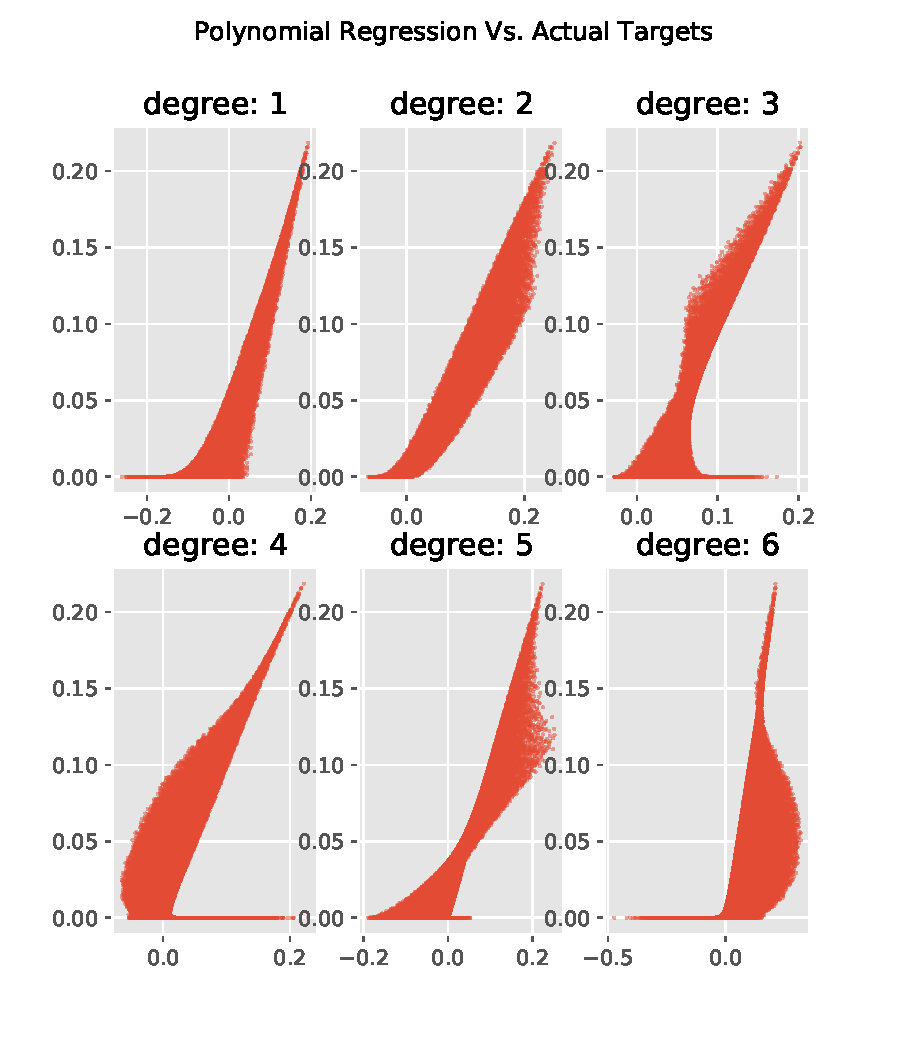
\includegraphics{Figures/polynomialOutMoneyEuroC.png}
\decoRule
\caption[Polynomial Regression Performance for out-of-money data set European Call]{Polynomial Regression Performance for out of money data set on the European call}
\label{fig:MLPsEuroCOutOfMoney}
\end{figure}

\begin{figure}[th]
\centering
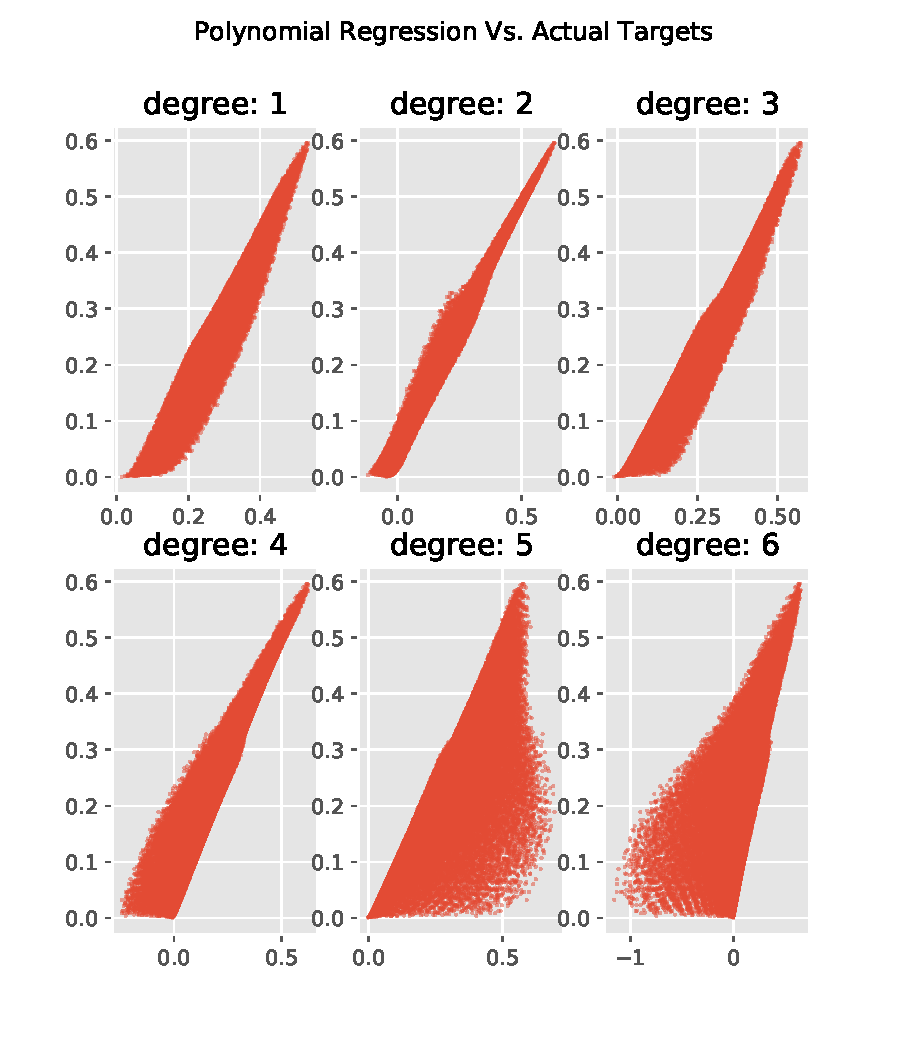
\includegraphics{Figures/polynomialLongTEuroC.png}
\decoRule
\caption[Polynomial Regression Performance for long maturity data set European call]{Polynomial Regression Performance for long maturity data set on European call}
\label{fig:MLPsEuroCLongMaturity}
\end{figure}


\begin{figure}[th]
\centering
\includegraphics{Figures/outMoneyAmerP.png}
\decoRule
\caption[MLPs Performance for In-the-Money data set on American Put]{MLPs Performance for In-the-Money data set on American Put}
\label{fig:MLPsAmerPOutMoney}
\end{figure}

\begin{figure}[th]
\centering
\includegraphics{Figures/longTAmerP.png}
\decoRule
\caption[MLPs Performance for long maturity data set on American Put]{MLPs Performance for long maturity data set on American Put}
\label{fig:MLPsAmerPLongT}
\end{figure}

\begin{figure}[th]
\centering
\includegraphics{Figures/longTAmerMinP.png}
\decoRule
\caption[MLPs Performance on long maturity data set on American bivariate contingent claim]{MLPs Performance for long maturity data set on American put on minimum of two stocks}
\label{fig:MLPsAmerMin1}
\end{figure}


\begin{figure}[th]
\centering
\includegraphics{Figures/inMoneyAmerMinP.png}
\decoRule
\caption[MLPs Performance on In-the-Money data set on American bivariate contingent claim]{MLPs Performance on In-the-Money data set on American put on minimum of two stocks}
\label{fig:MLPsAmerMin2}
\end{figure}



